\documentclass[8pt, xcolor={svgnames}, hyperref={linkcolor=black}]{beamer}
\usepackage[labelfont={color=amethyst,bf}]{caption}
\setbeamercolor{background canvas}{bg=white}
\usetheme[progressbar=frametitle]{metropolis}
\usepackage{appendixnumberbeamer}
\usepackage{url}
\usepackage{booktabs}
\usepackage{braket}
\usepackage[scale=2]{ccicons}
\usepackage{amsfonts} 
\usepackage{amssymb}
\usepackage[english]{babel}
\colorlet{col1}{teal}
\colorlet{col2}{yellow}
\colorlet{col3}{green}
\usepackage{fontawesome}
\usepackage{subcaption}
\usepackage{multicol}
\usepackage{bm}
\usepackage{algorithm}
\usepackage{algpseudocode}
\usepackage{enumitem}

\usepackage[]{pseudo}


\usepackage{tikz}
\usetikzlibrary{positioning,arrows,calc,math,angles,quotes}
\usepackage{blochsphere}

\usetikzlibrary{arrows,automata}
\usetikzlibrary{positioning}
\usetikzlibrary{arrows.meta,
                bending,
                intersections,
                quotes,
                shapes.geometric}

\tikzset{
    state/.style={
           rectangle,
           rounded corners,
           draw=black, very thick,
           minimum height=1em,
           inner sep=2pt,
           text centered,
           },
}


\definecolor{myv}{rgb}{0.36, 0.22, 0.33}
\definecolor{gio}{rgb}{0.45, 0.31, 0.59}
\definecolor{light}{rgb}{0.8, 0.8, 1}
\definecolor{warmblack}{rgb}{0.0, 0.26, 0.26}
\definecolor{brown(web)}{rgb}{0.65, 0.16, 0.16}
\definecolor{cadmiumgreen}{rgb}{0.0, 0.42, 0.24}
\definecolor{darkmidnightblue}{rgb}{0.0, 0.2, 0.4}
\definecolor{brightube}{rgb}{0.82, 0.62, 0.91}

\definecolor{codegreen}{rgb}{0,0.6,0}
\definecolor{codegray}{rgb}{0.5,0.5,0.5}
\definecolor{codepurple}{rgb}{0.58,0,0.82}
\definecolor{backcolour}{rgb}{0.95,0.95,0.92}
\definecolor{amethyst}{rgb}{0.6, 0.33, 0.73}

\definecolor{light-gray}{gray}{0.95}
\newcommand{\code}[1]{\colorbox{light-gray}{\texttt{#1}}}

\usepackage[most]{tcolorbox}
\usepackage{xcolor}

%\usepackage[citecolor = green, linkcolor = blue, bookmarks=true, urlcolor=blue,
%colorlinks=true, pagebackref=true]{hyperref}


%\usepackage{xspace}

\title{Full-stack Quantum Machine Learning for HEP}
\subtitle{MCM23}
\date{20 December 2023}
\author[Matteo Robbiati]{Matteo Robbiati}
\titlegraphic{
\begin{tikzpicture}[overlay, remember picture]

\node[at=(current page.south east), anchor=south east] {%
\includegraphics[width=.18\textwidth]{figures/qibo.png} 

\includegraphics[width=.18\textwidth]{figures/unimi.png} 
\includegraphics[width=.18\textwidth]{figures/cern.png}  
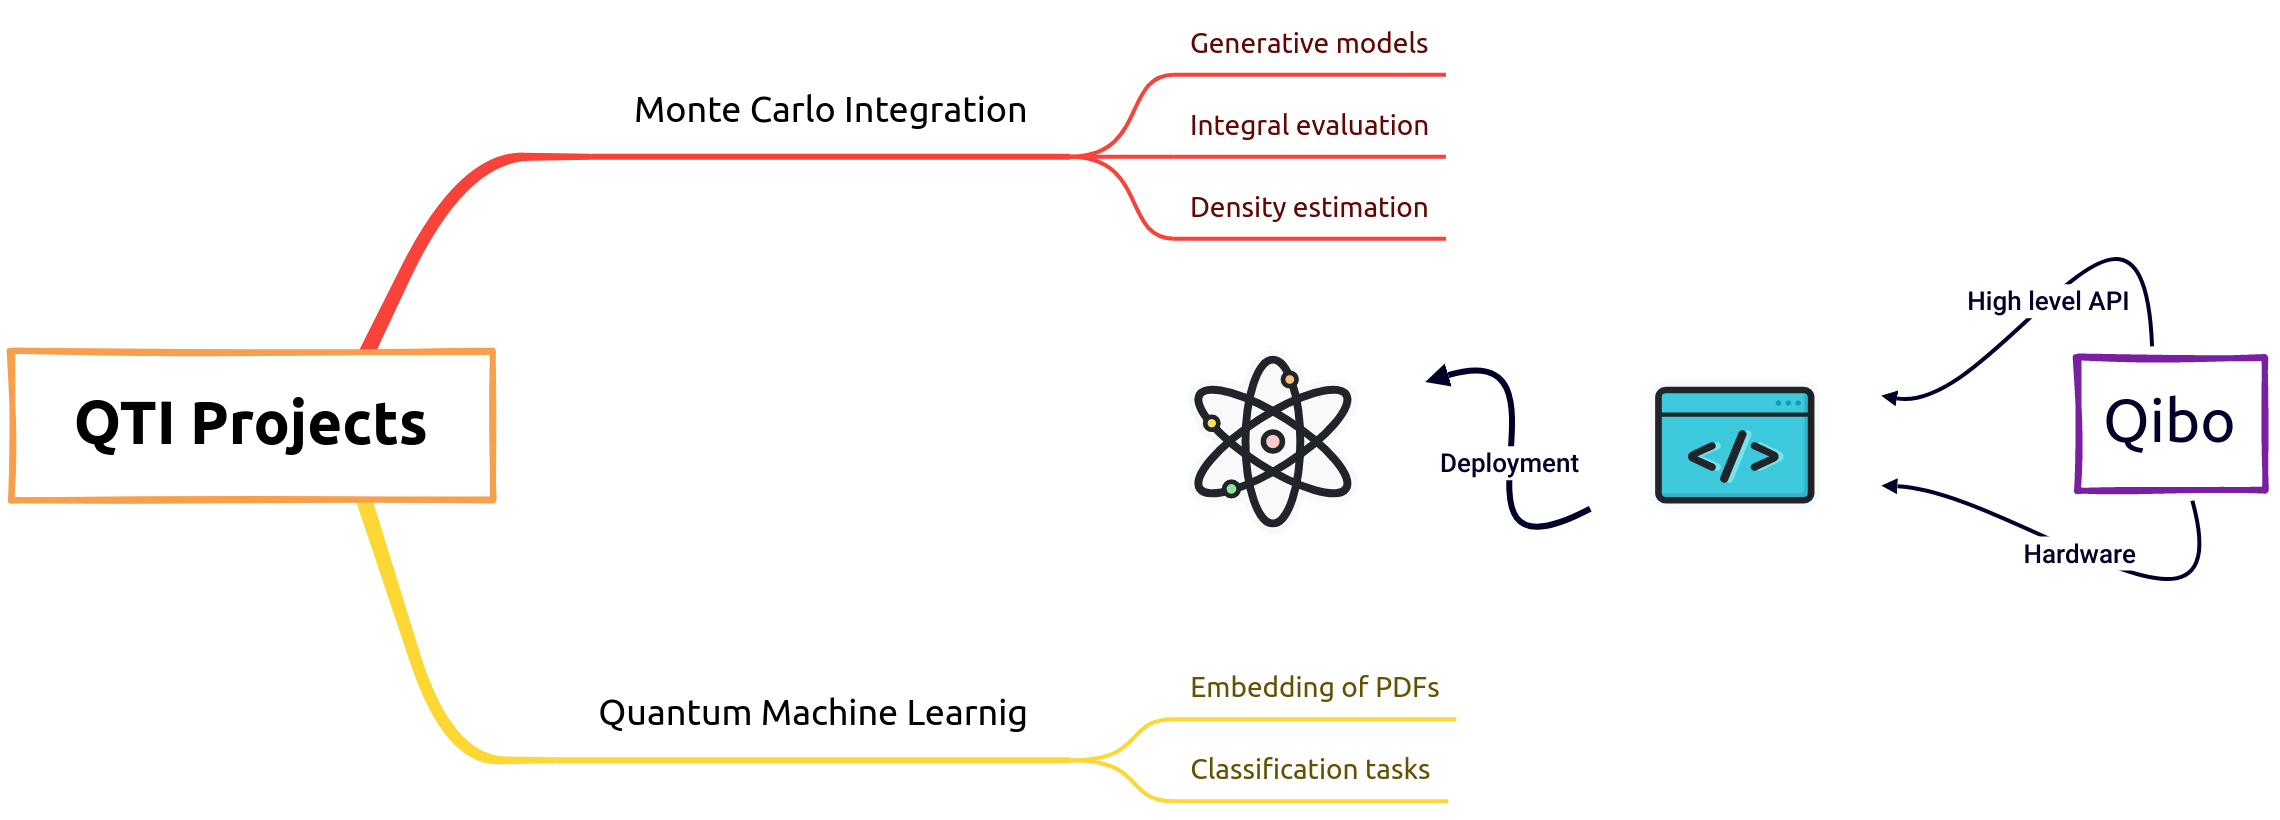
\includegraphics[width=.18\textwidth]{figures/qti.png}  
};
\end{tikzpicture}
}


\begin{document}

\maketitle

\begin{frame}{Aim and motivation}
\begin{figure}  
    \includegraphics[width=0.8\textwidth]{figures/motivation.png}
\end{figure}
\end{frame}

\section{Introductory concepts}

\begin{frame}{Machine Learning}
\vspace{0.5cm}
Machine Learning helps in solving statistical problems, such as data generation, 
classification, regression, forecasting, etc.
\pause

\begin{itemize}
\item[\faCrosshairs] we aim to know some hidden law between two variables: $\bm{y}=f(\bm{x})$;
\pause
\item[\faBarChart] we define a parameteric model with returns $\bm{y}_{\rm est}=f_{\rm est}(\bm{x}; \bm{\theta})$;
\pause
\item[\faBinoculars] we define an optimizer, which task is to compute 
   $\text{argmin}_{\bm{\theta}}\bigl[J(\bm{y}_{\rm meas}, \bm{y}_{\rm est})\bigr]$.
\end{itemize}
\pause
\begin{figure}  
    \includegraphics[width=1\textwidth]{figures/ml_scheme.png}
\end{figure}
\end{frame}

\begin{frame}{Parametric Quantum Circuits}
\pause
  \begin{itemize}
  \item<2,3,4>[\faMagic] Classical bits are replaced by \textbf{qubits}: 
  $\ket{q}=\alpha_0 \ket{0} + \alpha_1 \ket{1}$;  
  \item<3,4>[\faCog] we modify the qubits state by applying unitaries, which we call \textbf{gates}.\\
  Rotational gates $R_j(\theta)=e^{-i\theta\hat{\sigma}_j}$ are used to build
  parametric circuits $\mathcal{C}(\bm{\theta})$;
  \item<4>[\faEye] information is accessed calculating expected values $\text{E}[\hat{O}\,]$
  of target observables $\hat{O}$ on the state obtained executing $\mathcal{C}$.
  \end{itemize}
    \begin{figure}
       \includegraphics<2>[width=0.8\textwidth]{figures/vqc_1.png}
       \includegraphics<3>[width=0.8\textwidth]{figures/vqc_2.png}
       \includegraphics<4>[width=0.8\textwidth]{figures/vqc.png}   
    \end{figure}
\end{frame}

% SLIDE 1 QML
\begin{frame}{Quantum Machine Learning - doing ML using QC}

\vspace{1.05cm}

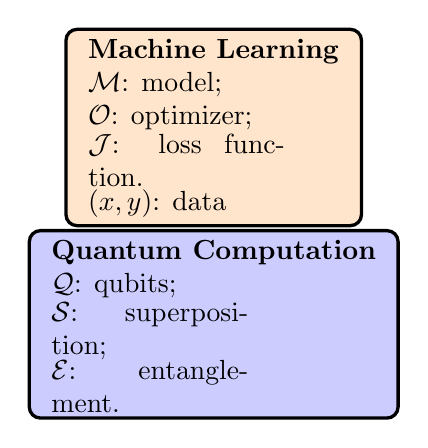
\begin{tikzpicture}[->,>=stealth']

 \node[state, fill=orange!20] (ML) 
 {\begin{tabular}{l}
 \textbf{Machine Learning}\\ 
 \parbox{2.5cm}{$\mathcal{M}$: model;}\\
 \parbox{2.5cm}{$\mathcal{O}$: optimizer;}\\
 \parbox{2.5cm}{$\mathcal{J}$: loss function.}\\
 \parbox{2.5cm}{$(x, y)$: data}
  \end{tabular}
  };
  
  \node[state,
  below of = ML,
  yshift=-1.5cm, fill=blue!20] (QC) 
 {\begin{tabular}{l}
 \textbf{Quantum Computation}\\ 
 \parbox{2.5cm}{$\mathcal{Q}$: qubits;} \\
 \parbox{2.5cm}{$\mathcal{S}$: superposition;}\\
 \parbox{2.5cm}{$\mathcal{E}$: entanglement.}
  \end{tabular}
  };
  
\end{tikzpicture}
\end{frame}


% SLIDE 2 QML
\begin{frame}{Quantum Machine Learning - operating on qubits}

\vspace{1.77cm}

\begin{tikzpicture}[->,>=stealth']

 \node[state, fill=orange!20] (ML) 
 {\begin{tabular}{l}
 \textbf{Machine Learning}\\ 
 \parbox{2.5cm}{$\mathcal{M}$: model;}\\
 \parbox{2.5cm}{$\mathcal{O}$: optimizer;}\\
 \parbox{2.5cm}{$\mathcal{J}$: loss function.}\\
 \parbox{2.5cm}{$(x, y)$: data}
  \end{tabular}
  };
  
  \node[state,
  below of = ML,
  yshift=-1.5cm, fill=blue!20] (QC) 
 {\begin{tabular}{l}
 \textbf{Quantum Computation}\\ 
 \parbox{2.5cm}{$\mathcal{Q}$: qubits;} \\
 \parbox{2.5cm}{$\mathcal{S}$: superposition;}\\
 \parbox{2.5cm}{$\mathcal{E}$: entanglement.}
  \end{tabular}
  };
  
 \node[state,
    right of=QC,
    yshift=-0.5cm,
    anchor=center,
    node distance=4.5cm, 	
    text width=3.5cm, fill=blue!20] (VQC) 
 {%
 \begin{tabular}{l}
  \textbf{Circuit execution} \\
  \parbox{4.5cm}{
  \includegraphics[width=0.9\textwidth]{figures/vqc.png}
  }
 \end{tabular}
 };
 
  \draw[line width=0.3mm] (1, -2.5)  to[out=0, in=200] (3, -3.2);
\end{tikzpicture}

\end{frame}

% SLIDE 3 QML
\begin{frame}{Quantum Machine Learning - natural randomness}

\vspace{1.77cm}

\begin{tikzpicture}[->,>=stealth']

 \node[state, fill=orange!20] (ML) 
 {\begin{tabular}{l}
 \textbf{Machine Learning}\\ 
 \parbox{2.5cm}{$\mathcal{M}$: model;}\\
 \parbox{2.5cm}{$\mathcal{O}$: optimizer;}\\
 \parbox{2.5cm}{$\mathcal{J}$: loss function.}\\
 \parbox{2.5cm}{$(x, y)$: data}
  \end{tabular}
  };
  
  \node[state,
  below of = ML,
  yshift=-1.5cm, fill=blue!20] (QC) 
 {\begin{tabular}{l}
 \textbf{Quantum Computation}\\ 
 \parbox{2.5cm}{$\mathcal{Q}$: qubits;} \\
 \parbox{2.5cm}{$\mathcal{S}$: superposition;}\\
 \parbox{2.5cm}{$\mathcal{E}$: entanglement.}
  \end{tabular}
  };
  
 \node[state,
    right of=QC,
    yshift=-0.5cm,
    anchor=center,
    node distance=4.5cm, 	
    text width=3.5cm, fill=blue!20] (VQC) 
 {%
 \begin{tabular}{l}
  \textbf{Circuit execution} \\
  \parbox{4.5cm}{
  \includegraphics[width=0.9\textwidth]{figures/vqc.png}
  }
 \end{tabular}
 };
 
\node[state,
  right of = VQC,
  node distance = 3cm,
  yshift=2cm, 
  fill=blue!20] (NSHOT) 
 {\begin{tabular}{l}
 \textbf{Expected values}\\ 
 $y_{est} \equiv \braket{q_f|\hat{O}|q_f}$
  \end{tabular}
  };
 
\draw[line width=0.3mm] (1, -2.5)  to[out=0, in=200] (3, -3.2);
\draw[line width=0.3mm] (6, -2.8)  to[out=0, in=250] (7, -1.6);
\end{tikzpicture}

\end{frame}


% SLIDE 4 QML
\begin{frame}{Quantum Machine Learning - encoding the problem}

\vspace{0.56cm}
\begin{tikzpicture}[->,>=stealth']

 \node[state, fill=orange!20] (ML) 
 {\begin{tabular}{l}
 \textbf{Machine Learning}\\ 
 \parbox{2.5cm}{$\mathcal{M}$: model;}\\
 \parbox{2.5cm}{$\mathcal{O}$: optimizer;}\\
 \parbox{2.5cm}{$\mathcal{J}$: loss function.}\\
 \parbox{2.5cm}{$(x, y)$: data}
  \end{tabular}
  };
  
  \node[state,
  below of = ML,
  yshift=-1.5cm, fill=blue!20] (QC) 
 {\begin{tabular}{l}
 \textbf{Quantum Computation}\\ 
 \parbox{2.5cm}{$\mathcal{Q}$: qubits;} \\
 \parbox{2.5cm}{$\mathcal{S}$: superposition;}\\
 \parbox{2.5cm}{$\mathcal{E}$: entanglement.}
  \end{tabular}
  };
  
 
 \node[state,
    right of=QC,
    yshift=-0.5cm,
    anchor=center,
    node distance=4.5cm, 	
    text width=3.5cm, fill=blue!20] (VQC) 
 {%
 \begin{tabular}{l}
  \textbf{Circuit execution} \\
  \parbox{4.5cm}{
  \includegraphics[width=0.9\textwidth]{figures/vqc.png}
  }
 \end{tabular}
 };
 
\node[state,
  right of = VQC,
  node distance = 3cm,
  yshift=2cm, 
  fill=blue!20] (NSHOT) 
 {\begin{tabular}{l}
 \textbf{Expected values}\\ 
 $y_{est} \equiv \braket{q_f|\hat{O}|q_f}$
  \end{tabular}
  };

  
 \draw[line width=0.3mm, red, opacity = 0.7] (0.5, 0.4)  to[out=0, in=230] (3, -3.3);
 \draw[line width=0.3mm, orange, opacity = 0.7] (-1.2, -1.25)  to[out=260, in=300] (4.4, -4.1);
 \draw[line width=0.3mm, cadmiumgreen, opacity = 0.7] (-0.4, -1.2)  to[out=330, in=80] (7.8, -0.4);
  
 
 \draw[red, line width=0.4mm, opacity = 0.9] (-1.1, 0.4) circle (0.4 cm);
 \draw[cadmiumgreen, line width=0.4mm, opacity = 0.9] (-0.65,-0.8) circle (0.3 cm);
 \draw[cadmiumgreen, line width=0.4mm, opacity = 0.9] (7.2,-1.4) rectangle (8.6, -0.95);
 \draw[orange, line width=0.4mm, opacity = 0.6] (-1.15,-0.8) circle (0.3 cm);
 \draw[red, line width=0.4mm, opacity = 0.6] (3.1,-4) rectangle (6,-2.4);
 \draw[orange, line width=0.4mm, opacity = 0.9] (3.5,-3.9) rectangle (5.2,-2.5);


\end{tikzpicture}
\end{frame}


% SLIDE 5 QML
\begin{frame}{Quantum Machine Learning!}

\vspace{0.42cm}
\begin{tikzpicture}[->,>=stealth']


 \node[state, fill=orange!20] (ML) 
 {\begin{tabular}{l}
 \textbf{Machine Learning}\\ 
 \parbox{2.5cm}{$\mathcal{M}$: model;}\\
 \parbox{2.5cm}{$\mathcal{O}$: optimizer;}\\
 \parbox{2.5cm}{$\mathcal{J}$: loss function.}\\
 \parbox{2.5cm}{$(x, y)$: data}
  \end{tabular}
  };
  
  \node[state,
  below of = ML,
  yshift=-1.5cm, fill=blue!20] (QC) 
 {\begin{tabular}{l}
 \textbf{Quantum Computation}\\ 
 \parbox{2.5cm}{$\mathcal{Q}$: qubits;} \\
 \parbox{2.5cm}{$\mathcal{S}$: superposition;}\\
 \parbox{2.5cm}{$\mathcal{E}$: entanglement.}
  \end{tabular}
  };
  

 \node[state,   
  text width=3cm, 
  yshift=1.5cm, 
  right of=ML, 	
  node distance=4cm, 
  anchor=center, fill=green!20] (OPT) 
 {%
 \begin{tabular}{l} 	% content
  \textbf{Optimizer $\mathcal{O}$}\\
  Hybrid-strategy
 \end{tabular}
 };
 
 \node[state,
    right of=QC,
    yshift=-0.5cm,
    anchor=center,
    node distance=4.5cm, 	
    text width=3.5cm, fill=blue!20] (VQC) 
 {%
 \begin{tabular}{l}
  \textbf{Circuit execution} \\
  \parbox{4.5cm}{
  \includegraphics[width=0.9\textwidth]{figures/vqc.png}
  }
 \end{tabular}
 };
 
\node[state,
  right of = VQC,
  node distance = 3cm,
  yshift=2cm, 
  fill=blue!20] (NSHOT) 
 {\begin{tabular}{l}
 \textbf{Expected values}\\ 
 $y_{est} \equiv \braket{q_f|\hat{O}|q_f}$
  \end{tabular}
  };
  
  \node[state,
  above of = NSHOT,
  node distance = 1.5cm,
  yshift=0cm, fill=green!20] (J) 
 {\begin{tabular}{l}
 \textbf{loss function $\mathcal{J}$}\\ 
 $\mathcal{J}(y_{meas}, y_{est})$
  \end{tabular}
  };
  

 \draw[line width=0.3mm] (6.5, -3)  to[out=0, in=270] (7.5, -1.6);
 \draw[line width=0.3mm] (6, -1.1)  to[out=180, in=200] (6.1, 0.2);
 \draw[line width=0.3mm] (7.5, 1.1)  to[out=90, in=0] (5.7, 1.5);
 \draw[line width=0.6mm, opacity=0.8] (2, 1.6)  to[out=180, in=270] (-0.2, 2.9);
 
 \draw[line width=0.3mm, orange, opacity = 0.0] (-1.2, -1.25)  to[out=260, in=300] (4.4, -3.5);

\end{tikzpicture}
\end{frame}

\begin{frame}{From ML to QML}
\begin{figure}  
   \includegraphics[width=1\textwidth]{figures/qml_scheme.png}
\end{figure}
\end{frame}


\begin{frame}
\centering
\Large Thank you for your attention!
\end{frame}

\end{document}
